\documentclass[12pt]{article}
\usepackage{amsmath}
\usepackage{booktabs}
\usepackage{tabularx}
\usepackage{caption}
\usepackage{nameref}
\usepackage{graphicx}
\usepackage{float}

\title{The use of Multiple Measurements in Taxonomic Problems}
\author{R. A. Fisher, Sc.D., F.R.S.}
\date{}

\renewcommand{\thetable}{\Roman{table}}
\makeatletter
\renewcommand{\@seccntformat}[1]{\csname the#1\endcsname\hspace{0.5em}}
\makeatother

\begin{document}

\maketitle

\begin{abstract}
This was written to embody the working of a practical numerical example arising in plant taxonomy, in which the concept of a discriminant function seems to be of immediate service.\end{abstract}

\section{Discriminant Functions}

When two or more populations have been measured in several characters, $x_1, \dots, x_s$ special interest attaches to certain linear functions of the measurements by which the populations are best discriminated. At the author's suggestion use has already been made of this fact in craniometry ($a$) by Mr E. S. Martin, who has applied the principle to the sex differences in measurements of the mandible, and ($b$) by Miss Mildred Barnard, who showed how to obtain from a series of dated series the particular compound of cranial measurements showing most distinctly a progressive or secular trend. In the present paper the application of the same principle will be illustrated on a taxonomic problem; some questions connected with the precision of the processes employed will also be discussed.

\section{Arithmetical Procedure}

Table~\ref{tab:1} shows measurements of the flowers of fifty plants each of the two species \textit{Iris setosa} and \textit{I. versicolor}, found growing together in the same colony and measured by Dr E. Anderson, to whom I am indebted for the use of the data. Four flower measurements are given.

{
\setlength{\tabcolsep}{3pt}
\begin{table}[H]
\centering
\scriptsize
\caption{}
\label{tab:1}
\begin{tabularx}{\textwidth}{|*{12}{>{\centering\arraybackslash}X|}}
\hline
\multicolumn{4}{|c|}{\textit{Iris setosa}} &
\multicolumn{4}{c|}{\textit{Iris versicolor}} &
\multicolumn{4}{c|}{\textit{Iris virginica}} \\
\hline
Sepal length & Sepal width & Petal length & Petal width &
Sepal length & Sepal width & Petal length & Petal width &
Sepal length & Sepal width & Petal length & Petal width \\
\hline

5.1 & 3.5 & 1.4 & 0.2 & 7.0 & 3.2 & 4.7 & 1.4 & 6.3 & 3.3 & 6.0 & 2.5 \\
4.9 & 3.0 & 1.4 & 0.2 & 6.4 & 3.2 & 4.5 & 1.5 & 5.8 & 2.7 & 5.1 & 1.9 \\
4.7 & 3.2 & 1.3 & 0.2 & 6.9 & 3.1 & 4.9 & 1.5 & 7.1 & 3.0 & 5.9 & 2.1 \\
4.6 & 3.1 & 1.5 & 0.2 & 5.5 & 2.3 & 4.0 & 1.3 & 6.3 & 2.9 & 5.6 & 1.8 \\
5.0 & 3.6 & 1.4 & 0.2 & 6.5 & 2.8 & 4.6 & 1.5 & 6.5 & 3.0 & 5.8 & 2.2 \\
5.4 & 3.9 & 1.7 & 0.4 & 5.7 & 2.8 & 4.5 & 1.3 & 7.6 & 3.0 & 6.6 & 2.1 \\
4.6 & 3.4 & 1.4 & 0.3 & 6.3 & 3.3 & 4.7 & 1.6 & 4.9 & 2.5 & 4.5 & 1.7 \\
5.0 & 3.4 & 1.5 & 0.2 & 4.9 & 2.4 & 3.3 & 1.0 & 7.3 & 2.9 & 6.3 & 1.8 \\
4.4 & 2.9 & 1.4 & 0.2 & 6.6 & 2.9 & 4.6 & 1.3 & 6.7 & 2.5 & 5.8 & 1.8 \\
4.9 & 3.1 & 1.5 & 0.1 & 5.2 & 2.7 & 3.9 & 1.4 & 7.2 & 3.6 & 6.1 & 2.5 \\
5.4 & 3.7 & 1.5 & 0.2 & 5.0 & 2.0 & 3.5 & 1.0 & 6.5 & 3.2 & 5.1 & 2.0 \\
4.8 & 3.4 & 1.6 & 0.2 & 5.9 & 3.0 & 4.2 & 1.5 & 6.4 & 2.7 & 5.3 & 1.9 \\
4.8 & 3.0 & 1.4 & 0.1 & 6.0 & 2.2 & 4.0 & 1.0 & 6.8 & 3.0 & 5.5 & 2.1 \\
4.3 & 3.0 & 1.1 & 0.1 & 6.1 & 2.9 & 4.7 & 1.4 & 5.7 & 2.5 & 5.0 & 2.0 \\
5.8 & 4.0 & 1.2 & 0.2 & 5.6 & 2.9 & 3.6 & 1.3 & 5.8 & 2.8 & 5.1 & 2.4 \\
5.7 & 4.4 & 1.5 & 0.4 & 6.7 & 3.1 & 4.4 & 1.4 & 6.4 & 3.2 & 5.3 & 2.3 \\
5.4 & 3.9 & 1.3 & 0.4 & 5.6 & 3.0 & 4.5 & 1.5 & 6.5 & 3.0 & 5.5 & 1.8 \\
5.1 & 3.5 & 1.4 & 0.3 & 5.8 & 2.7 & 4.1 & 1.0 & 7.7 & 3.8 & 6.7 & 2.2 \\
5.7 & 3.8 & 1.7 & 0.3 & 6.2 & 2.2 & 4.5 & 1.5 & 7.7 & 2.6 & 6.9 & 2.3 \\
5.1 & 3.8 & 1.5 & 0.3 & 5.6 & 2.5 & 3.9 & 1.1 & 6.0 & 2.2 & 5.0 & 1.5 \\
5.4 & 3.4 & 1.7 & 0.2 & 5.9 & 3.2 & 4.8 & 1.8 & 6.9 & 3.2 & 5.7 & 2.3 \\
5.1 & 3.7 & 1.5 & 0.4 & 6.1 & 2.8 & 4.0 & 1.3 & 5.6 & 2.8 & 4.9 & 2.0 \\
4.6 & 3.6 & 1.0 & 0.2 & 6.3 & 2.5 & 4.9 & 1.5 & 7.7 & 2.8 & 6.7 & 2.0 \\
5.1 & 3.3 & 1.7 & 0.5 & 6.1 & 2.8 & 4.7 & 1.2 & 6.3 & 2.7 & 4.9 & 1.8 \\
4.8 & 3.4 & 1.9 & 0.2 & 6.4 & 2.9 & 4.3 & 1.3 & 6.7 & 3.3 & 5.7 & 2.1 \\
5.0 & 3.0 & 1.6 & 0.2 & 6.6 & 3.0 & 4.4 & 1.4 & 7.2 & 3.2 & 6.0 & 1.8 \\
5.0 & 3.4 & 1.6 & 0.4 & 6.8 & 2.8 & 4.8 & 1.4 & 6.2 & 2.8 & 4.8 & 1.8 \\
5.2 & 3.5 & 1.5 & 0.2 & 6.7 & 3.0 & 5.0 & 1.7 & 6.1 & 3.0 & 4.9 & 1.8 \\
5.2 & 3.4 & 1.4 & 0.2 & 6.0 & 2.9 & 4.5 & 1.5 & 6.4 & 2.8 & 5.6 & 2.1 \\
4.7 & 3.2 & 1.6 & 0.2 & 5.7 & 2.6 & 3.5 & 1.0 & 7.2 & 3.0 & 5.8 & 1.6 \\
4.8 & 3.1 & 1.6 & 0.2 & 5.5 & 2.4 & 3.8 & 1.1 & 7.4 & 2.8 & 6.1 & 1.9 \\
5.4 & 3.4 & 1.5 & 0.4 & 5.5 & 2.4 & 3.7 & 1.0 & 7.9 & 3.8 & 6.4 & 2.0 \\
5.2 & 4.1 & 1.5 & 0.1 & 5.8 & 2.7 & 3.9 & 1.2 & 6.4 & 2.8 & 5.6 & 2.2 \\
5.5 & 4.2 & 1.4 & 0.2 & 6.0 & 2.7 & 5.1 & 1.6 & 6.3 & 2.8 & 5.1 & 1.5 \\
4.9 & 3.1 & 1.5 & 0.1 & 5.4 & 3.0 & 4.5 & 1.5 & 6.1 & 2.6 & 5.6 & 1.4 \\
5.0 & 3.2 & 1.2 & 0.2 & 6.0 & 3.4 & 4.5 & 1.6 & 7.7 & 3.0 & 6.1 & 2.3 \\
5.5 & 3.5 & 1.3 & 0.2 & 6.7 & 3.1 & 4.7 & 1.5 & 6.3 & 3.4 & 5.6 & 2.4 \\
4.9 & 3.1 & 1.5 & 0.1 & 6.3 & 2.3 & 4.4 & 1.3 & 6.4 & 3.1 & 5.5 & 1.8 \\
4.4 & 3.0 & 1.3 & 0.2 & 5.6 & 3.0 & 4.1 & 1.3 & 6.0 & 3.0 & 4.8 & 1.8 \\
5.1 & 3.4 & 1.5 & 0.2 & 5.5 & 2.5 & 4.0 & 1.3 & 6.9 & 3.1 & 5.4 & 2.1 \\
5.0 & 3.5 & 1.3 & 0.3 & 5.5 & 2.6 & 4.4 & 1.2 & 6.7 & 3.1 & 5.6 & 2.4 \\
4.5 & 2.3 & 1.3 & 0.3 & 6.1 & 3.0 & 4.6 & 1.4 & 6.9 & 3.1 & 5.1 & 2.3 \\
4.4 & 3.2 & 1.3 & 0.2 & 5.8 & 2.6 & 4.0 & 1.2 & 5.8 & 2.7 & 5.1 & 1.9 \\
5.0 & 3.5 & 1.6 & 0.6 & 5.0 & 2.3 & 3.3 & 1.0 & 6.8 & 3.2 & 5.9 & 2.3 \\
5.1 & 3.8 & 1.9 & 0.4 & 5.6 & 2.7 & 4.2 & 1.3 & 6.7 & 3.3 & 5.7 & 2.5 \\
4.8 & 3.0 & 1.4 & 0.3 & 5.7 & 3.0 & 4.2 & 1.2 & 6.7 & 3.0 & 5.2 & 2.3 \\
5.1 & 3.8 & 1.6 & 0.2 & 5.7 & 2.9 & 4.2 & 1.3 & 6.3 & 2.5 & 5.0 & 1.9 \\
4.6 & 3.2 & 1.4 & 0.2 & 6.2 & 2.9 & 4.3 & 1.3 & 6.5 & 3.0 & 5.2 & 2.0 \\
5.3 & 3.7 & 1.5 & 0.2 & 5.1 & 2.5 & 3.0 & 1.1 & 6.2 & 3.4 & 5.4 & 2.3 \\
5.0 & 3.3 & 1.4 & 0.2 & 5.7 & 2.8 & 4.1 & 1.3 & 5.9 & 3.0 & 5.1 & 1.8 \\
\hline
\end{tabularx}
\end{table}
}

We shall first consider the question: What linear function of the four measurements
\[
X = \lambda_{1} x_{1} + \lambda_{2} x_{2} + \lambda_{3} x_{3} + \lambda_{4} x_{4}
\]
will maximize the ratio of the difference between the specific means to the standard deviations within species? The observed means and their differences are shown in Table~\ref{tab:2}. We may represent the differences by $d_p$, where \text{$p = 1,\,2,\,3 \text{ or } 4$} for the four measurements.

\begin{table}[H]
\centering
\footnotesize
\caption[Statistical Methods]{Observed means for two species and their difference (cm.)}
\label{tab:2}
\begin{tabularx}{\textwidth}{|>{\centering\arraybackslash}X
                               |>{\centering\arraybackslash}X
                               |>{\centering\arraybackslash}X
                               |>{\centering\arraybackslash}X|}
\hline
 & Versicolor & Setosa & Difference ($V-S$) \\
\hline
Sepal length ($x_1$) & 5.936 & 5.006 & 0.930 \\
Sepal width ($x_2$)  & 2.770 & 3.428 & $-0.658$ \\
Petal length ($x_3$) & 4.260 & 1.462 & 2.798 \\
Petal width ($x_4$)  & 1.326 & 0.246 & 1.080 \\
\hline
\end{tabularx}
\end{table}

The sums of squares and products of deviations from the specific means are shown in Table~\ref{tab:3}. Since fifty plants of each species were used these sums contain 98 degrees of freedom. We may represent these sums of squares or products by $S_{pq}$, where $p$ and $q$ take independently the values \text{$1,\,2,\,3 \text{ and } 4$}.

\begin{table}[H]
\centering
\footnotesize
\caption{Sums of squares and products of four measurements, within species (cm$^2$).}
\label{tab:3}
\begin{tabularx}{\textwidth}{|*{5}{>{\centering\arraybackslash}X|}}
\hline
 & Sepal length & Sepal width & Petal length & Petal width \\
\hline
Sepal length & 19.1434 & 9.0356  & 9.7634  & 3.2394 \\
Sepal width  & 9.0356  & 11.8658 & 4.6232  & 2.4746 \\
Petal length & 9.7634  & 4.6232  & 12.2978 & 3.8794 \\
Petal width  & 3.2394  & 2.4746  & 3.8794  & 2.4604 \\
\hline
\end{tabularx}
\end{table}

Then for any linear function, $X$, of the measurements, as defined above, the difference between the means of $X$ in the two species is

\[
D = \lambda_{1} d_{1} + \lambda_{2} d_{2} + \lambda_{3} d_{3} + \lambda_{4} d_{4}
\] while the variance of $X$ within species is proportional to

\[
S = \sum_{p=1}^{4}\sum_{q=1}^{4} \lambda_{p} \lambda_{q} S_{pq}
\].

The particular linear finction which best discriminates the two species will be one for
which the ratio $D^2/S$ is greatest, by variation of the four coefficients $\lambda_{1}$,$\lambda_{2}$, $\lambda_{3}$ and $\lambda_{4}$ independently. This gives for each $\lambda$

\[
\frac{D}{S^2} \biggl\{ 2S \frac{\partial D}{\partial \lambda} - D \frac{\partial S}{\partial \lambda} \biggl\} = 0,
\] or

\[
\frac{1}{2} \frac{\partial S}{\partial \lambda} = 
\frac{S}{D} \frac{\partial D}{\partial \lambda},
\] where it may be noticed that $S/D$ is a factor constant for the four unknown coefficients. Consequently, the coefficients required are proportional to the solutions of the equations

\begin{equation} \label{eq:1}
\left.
\begin{aligned}
S_{11} \lambda_{1} + S_{12} \lambda_{2} + S_{13} \lambda_{3} + S_{14} \lambda_{4} &= d_1 ,\\
S_{21} \lambda_{1} + S_{22} \lambda_{2} + S_{23} \lambda_{3} + S_{24} \lambda_{4} &= d_2 ,\\
S_{31} \lambda_{1} + S_{32} \lambda_{2} + S_{33} \lambda_{3} + S_{34} \lambda_{4} &= d_3 ,\\
S_{41} \lambda_{1} + S_{42} \lambda_{2} + S_{43} \lambda_{3} + S_{44} \lambda_{4} &= d_4 .
\end{aligned}
\right\}
\end{equation}

If, in turn, unity is substituted for each of the differences and zero for the others, the solutions obtained constitute the matrix of multipliers reciprocal to the matrix of $S$; numerically we find:

\begin{table}[H]
\centering
\footnotesize
\caption{Matrix of multipliers reciprocal to the sums of squares and products within species (cm$^{-2}$).}
\label{tab:4}
\begin{tabularx}{\textwidth}{|*{5}{>{\centering\arraybackslash}X|}}
\hline
 & Sepal length & Sepal width & Petal length & Petal width \\
\hline
Sepal length &  0.1187161 & -0.0668666 & -0.0816158 &  0.0396350 \\
Sepal width  & -0.0668666 &  0.1452736 &  0.0334101 & -0.1107529 \\
Petal length & -0.0816158 &  0.0334101 &  0.2193614 & -0.2720206 \\
Petal width  &  0.0396350 & -0.1107529 & -0.2720206 &  0.8945506 \\
\hline
\end{tabularx}
\end{table}

These values may be denoted by $s_{pq}$ for values of $p$ and $q$ from l to 4.

Multiplying the columns of the matrix in Table~\ref{tab:4} by the observed differences, we have
the solutions of the equation \eqref{eq:1} in the form
\[
\lambda_{1}=-0.0311511, \lambda_{2}=-0.1839075, \lambda_{3}=+0.2221044, \lambda_{4}=+0.3147370,
\] so that, if we choose to take the coefficient of sepal length to be unity, the compound
measurement required is
\[
X = x_1 + 5.9037 x_2 - 7.1299 x_3 - 10.1036 x_4.
\] If in this expression we substitute the values observed in \textit{setosa} plants, the mean, as found
from the values in Table~\ref{tab:1}, is
\[
5.006 + (3.428)(5.9037) - (1.462)(7.1299) - (0.246)(10.1036) = 12.3345\ cm.;
\] for \textit{versicolor}, on the contrary, we have
\[
5.936 + (2.770)(5.9037) - (4.260)(7.1299) - (1.326)(10.1036) = -21.4815\ cm.
\] The difference between the average values of the compound measurements being thus
33.816 cm.

The distinctness of the metrical characters of the two species may now be gauged by
comparing this difference between the average values with its standard error. Using the
values of Table~\ref{tab:3}, with the coefficients of our compound, we have
{\small
\[
\begin{aligned}
19.1431 + (9.0356)(5.9037) - (9.7634)(7.1299) - (3.2394)(10.1036) &= -29.8508,\\
9.0356 + (11.8658)(5.9037) - (4.6232)(7.1299) - (2.4746)(10.1036) &= 21.1224,\\
9.7634 + (4.6232)(5.9037) - (12.2978)(7.1299) - (3.8794)(10.1036) &= -89.8206,\\
3.2394 + (2.4746)(5.9037) - (3.8794)(7.1299) - (2.4604)(10.1036) &= -34.6699,
\end{aligned}
\] } and finally,
{\small
\[
-29.8508 + (21.1224)(5.9037) + (89.8206)(7.1299) + (34.6699)(10.1036) = 1085.5522.
\] }

The average variance of the two species in respect of the compound measurements may
be estimated by dividing this value (1085.5522) by 95; the variance of the difference
between two means of fifty plants each, by dividing again by 25. For single plants the
variance is 11.4269, so that the mean difference, 33.816 cm., between a pair of plants of
different species has a standard deviation of 4.781 cm. For means of fifty the same average
difference has the standard error 0.6761 em., or only about one-fiftieth of its value.

\section{Interpretation}

The ratio of the difference between the means of the chosen compound measurement
to its standard error in individual plants is of interest also in relation to the probability
of misclassification, if the specific nature were judged wholly from the measurements.
For reasons to be discussed later we shall estimate the variance of a single plant by dividing
1085.5522 by 95, giving 11.4269 $cm^2$. for the variance, and 3.3804 cm. for the standard
deviation. Supposing that a plant is misclassified, if its deviation in the right direction
exceeds half the difference, 33.816 cm., between the species, the ratio to the standard as
estimated is 5.0018.

The table of the normal distribution (\textit{\nameref{tab:2}}, Table~\ref{tab:2}) shows that a ratio
4.89164 is exceeded five times in a million, and 5.32672 only once in two million trials.
By logarithmic interpolation the frequency appropriate to a ratio 5.0018 is about 2.79 per
million. If the variances of the two species are unequal, this frequenecy is somewhat
overestimated by this method, since we ought to divide the specific difference in proportion
to the two standard deviations, and for constant sum of variances the sum of the standard
deviations is greatest when they are equal. We may, therefore, at once conclude that if
the measurements are nearly normally distributed the probability of misclassification,
using the compound measurement only is less than three per million.

The same ratio is of interest from another aspect. If the chosen compound $X$ is analysed
in respect to its variation within and between species, the sum of squares between species
must be $25 D^2$. Numerically we have, therefore,

\begin{table}[H]
\centering
\footnotesize
\caption{Analysis of variance of the chosen compound $X$, between and within species}
\label{tab:5}
\begin{tabular}{|c|c|c|}
\hline
 & Degrees of freedom & Sum of squares \\
\hline
Between species & 4  & 28588.05 \\
Within species  & 95 & 1085.55  \\
\hline
Total           & 99 & 29673.60 \\
\hline
\end{tabular}
\end{table}

Of the total only 3.6583 per cent. is within species, and 96.3417 per cent. between species.
The compound has been chosen to maximize the latter percentage. Since, in addition to
the specific means, we have used three adjustable ratios, the variation within species
must contain only 95 degrees of freedom.

In making up the variate $X$, we have multiplied the original values of $\lambda$ by -32.1018
in order to give to the measurement sepal length the coefficient unity. Had we used the
original values, the analysis of Table~\ref{tab:5} would have appeared as:

\begin{table}[H]
\centering
\footnotesize
\caption{Analysis of variance of the crude compound $X$, between and within species}
\label{tab:6}
\begin{tabular}{|c|c|c|c|}
\hline
 & Degrees of freedom & Sum of squares & \\
\hline
Between species & 4  & 27.74160 & $=25 D^2$ \\
Within species  & 95 & 1.05341  & $=D=S$ \\
\hline
Total           & 99 & 28.79501 & $D(1+25D)$ \\
\hline
\end{tabular}
\end{table}

On multiplying equations \eqref{eq:1} by $\lambda_{1}$, $\lambda_{2}$, $\lambda_{3}$ and $\lambda_{4}$ and adding, it appears that
$S = \sum{\lambda d} = D$, the specific difference in the crude compound $X$.
The proportion (3.6 per cent.) of the sum of squares within species could therefore have been found simply as $1 / (1 + 25 D)$.

\section{The Analogy of Partial Regression}

The analysis of Table~\ref{tab:6} suggests an analogy of some interest. If to each plant were
assigned a value of a variate $y$, the same for all members of each species, the analysis of
variance of $y$, between the portions accountable by linear regression on the measurements
$x_{1}, \ldots, x_{4}$, and the residual variation after fitting such a regression, would be identical
with Table~\ref{tab:6}, if $y$ were given appropriate equal and opposite values for the two species.

In general, with different numbers of representatives of the two species, $n_{1}$ and $n_{2}$, if
the values of $y$ assigned were
\[
\frac{n_{2}}{n_{1}+n_{2}} \quad \text{and} \quad \frac{- n_{1}}{n_{1}+n_{2}},
\]
differing by unity, the right-hand sides of the equations for the regression coefficients,
corresponding to equation \eqref{eq:1}, would have been
\[
\frac{n_{1}n_{2}}{n_{1}+n_{2}} d_{p},
\]
where $d_{p}$ is the difference between the means of the two species in any one of the measurements. The typical coefficient of the left-hand side would be
\[
S_{pq} + \frac{n_{1}n_{2}}{n_{1}+n_{2}} d_{p} d_{q}.
\]

Transferring the additional fractions to the right-hand side, we should have equations
identical with \eqref{eq:1}, save that the right-hand sides are now
\[
\frac{n_{1}n_{2}}{n_{1}+n_{2}} d_{p} \, (1 - \sum \lambda' d),
\]
where $\lambda'$ stands for a solution of the new equations; hence
\[
\lambda' = \frac{n_{1}n_{2}}{n_{1}+n_{2}} (1 - \sum \lambda' d) \, \lambda,
\]
multiply these equations by $d$ and add, so that
\[
\sum \lambda' d = \frac{n_{1}n_{2}}{n_{1}+n_{2}} \sum \lambda d \, (1 - \sum \lambda' d),
\]
or
\[
(1 - \sum \lambda' d) \left( 1 + \frac{n_{1}n_{2}}{n_{1}+n_{2}} \sum \lambda d \right) = 1,
\]
and so in our example
\[
1 - \sum \lambda' d = \frac{1}{1+25D}.
\]

The analysis of variance of $y$ is, therefore,

\begin{table}[H]
\centering
\footnotesize
\caption{Analysis of variance of a variate $y$ determined exclusively by the species}
\label{tab:7}
\begin{tabular}{|c|c|c|c|}
\hline
 & Degrees of freedom & Sum of squares & \\
\hline
Regression & 4  & 24.0854 &  $ 25^2D/(1+25D)$ \\
Remainder  & 95 & 0.9146  &  $ 25/(1+25D)$ \\
\hline
Total      & 99 & 25.0000 & \\
\hline
\end{tabular}
\end{table}

The total $S (y^2)$ is clearly in general \(\frac{n_{1}n_{2}}{n_{1}+n_{2}}\); the portion ascribable to regression is

\[
\frac{n_{1}n_{2}}{n_{1}+n_{2}}\sum\lambda' d=\frac{25^{2}D}{1+25D}.
\]

In this method of presentation the appropriate allocation of the degrees of freedom is evident.

The multiple correlation of \(y\) with the measurements \(x_{1}\), \ldots, \(x_{4}\) is given by

\[
R^{2}=\frac{25D}{1+25D}.
\]

\section{Test of significance}

It is now clear in what manner the specific difference may be tested for significance, so as to allow for the fact that a variate has been chosen so as to maximise the distinctness of the species. The regression of \(y\) on the four measurements is given 4 degrees of freedom, and the residual variation 95; the value of $z$ calculated from the sums of squares in any one of Tables \ref{tab:5}, \ref{tab:6} or \ref{tab:7} is 3.2183 or
\[
\frac{1}{2} (\log\,95-\log\,4+\log\,25+\log\,D),
\]
a very significant value for the number of degrees of freedom used.

\section{Applications to the theory of allopolyploidy}

We may now consider one of the extensions of this procedure which are available when samples have been taken from more than two populations. The sample of the third species given in Table~\ref{tab:1}, \textit{Iris virginica}, differs from the two other samples in not being taken from the same natural colony as they were -- a circumstance which might considerably disturb both the mean values and their variabilities. It is of interest in association with \textit{I. setosa} and \textit{I. versicolor} in that Randoph (1934) has ascertained and Anderson has confirmed that, whereas \textit{I. setosa} is a ``diploid'' species with 38 chromosomes, \textit{I. virginica} is ``tetraploid'', with 70, and \textit{I. versicolor}, which is intermediate in three measurements, though not in sepal breadth, is hexaploid. He has suggested the interesting possibility that \textit{I. versicolor} is a polyploid hybrid of the two other species. We shall, therefore, consider whether, when we use the linear compound of the four measurements most appropriate for discriminating three such species, the mean value for \textit{I. versicolor} takes an intermediate value, and, if so, whether it differs twice as much from \textit{I. setosa} as from \textit{I. virginica}, as might be expected, if the effects of genes are simply additive, in a hybrid between a diploid and a tetraploid species.

If a third value lies two-thirds of the way from one value to another, the three deviations from their common mean must be in the ratio $4:1:-5$. To obtain values corresponding with the differences between the two species we may, therefore, form linear compounds of their mean measurements, using these numerical coefficients. The results are shown in Table~\ref{tab:8} where, for example, the value 7.258 cm. for sepal length is four times the mean 
sepal length for \textit{I. virginica} plus once the mean sepal length for \textit{I. versicolor} minus five times the value for \textit{I. setosa}.

\begin{table}[H]
\centering
\caption{}
\label{tab:8}
\begin{tabularx}{0.9\textwidth}{|*{5}{>{\centering\arraybackslash}X|}}
\hline
\text{Means} & \multicolumn{4}{|c|}{$S_{pq}$} \\
\hline
\multicolumn{5}{|c|}{\textit{Iris virginica}. Fifty plants} \\
\hline
6.588 & 19.8128 & 4.5944 & 14.8612 & 2.4056 \\
2.974 &  4.5944 & 5.0962 &  3.4976 & 2.3338 \\
5.552 & 14.8612 & 3.4976 & 14.9258 & 2.3924 \\
2.026 &  2.4056 & 2.3338 &  2.3924 & 3.6962 \\
\hline
\multicolumn{5}{|c|}{\textit{Iris versicolor}. Fifty plants} \\
\hline
5.936 & 13.0552 & 4.1740 &  8.9620 & 2.7332 \\
2.770 &  4.1740 & 4.8250 &  4.0500 & 2.0190 \\
4.260 &  8.9620 & 4.0500 & 10.8200 & 3.5820 \\
1.326 &  2.7332 & 2.0190 &  3.5820 & 1.9182 \\
\hline
\multicolumn{5}{|c|}{\textit{Iris setosa}. Fifty plants} \\
\hline
5.006 & 6.0882 & 4.8816 & 0.8014 & 0.5062 \\
3.428 & 4.8616 & 7.0408 & 0.5732 & 0.4556 \\
1.462 & 0.8014 & 0.5732 & 1.4778 & 0.2974 \\
0.246 & 0.5062 & 0.4556 & 0.2974 & 0.5442 \\
\hline
\multicolumn{5}{|c|}{ $4vi + ve - 5se$ } \\
\hline
 7.258 & 482.2650 & 199.2244 & 266.7762 & 53.8778 \\
-2.474 & 199.2244 & 262.3842 &  74.3416 & 50.7498 \\
19.158 & 266.7762 &  74.3416 & 286.6618 & 49.2954 \\
 8.200 &  53.8778 &  50.7498 &  49.2954 & 74.6604 \\
\hline
\end{tabularx}
\end{table}

Since the values for the sums of squares and products of deviations from the means within each of the three species are somewhat different, we may make an appropriate matrix corresponding with our chosen linear compound by multiplying the values for \textit{I. virginica} by 16, those for \textit{I. versicolor} by one and those for \textit{I. setosa} by 25, and adding the values for the three species, as shown in Table~\ref{tab:8}. The values so obtained will correspond with the matrix of sums of squares and products within species when only two populations have been sampled.

Using the rows of the matrix as the coefficients of four unknowns in an equation with our chosen compound of the mean measurements, e.g.

\[
482.2650 \lambda_1 + 199.2244 \lambda_2 + 266.7762 \lambda_3 + 53.8778 \lambda_4 = 7.258,
\]

we find solutions which, when multiplied by 100, are

\[
\begin{array}{cc}
\text{Coefficient of sepal length} & -3.308998 \\
\text{sepal breadth} & -2.759132 \\
\text{petal length} & 8.866048 \\
\text{petal breadth} & 9.392551 \\
\end{array}
\]

defining the compound measurement required.

It is now easy to find the means and variances of this compound measurement in the three species. These are shown in the table below (Table~\ref{tab:9}):

\begin{table}[H]
\centering
\caption{}
\label{tab:9}
\begin{tabularx}{\textwidth}{|l|*{4}{>{\centering\arraybackslash}X|}}
\hline
 & Mean & Sum of squares & Mean square & Standard deviation \\
\hline
\( I. virginica \) & 38.24827 & 923.7958 & 18.8530 & 4.342 \\
\( I. versicolor \) & 22.93888 & 873.5119 & 17.8268 & 4.222 \\
\( I. setosa \) & -10.75042 & 292.8958 & 5.9775 & 2.444 \\
\hline
\end{tabularx}
\end{table}

From this table it can be seen that, whereas the difference between \textit{I. setosa} and \textit{I. versicolor}, 33.69 of our units, is so great compared with the standard deviations that no appreciable overlapping of values can occur, the difference between \textit{I. virginica} and \textit{I. versicolor}, 15.31 units, is less than four times the standard deviation of each species.

The differences do seem, however, to be remarkably closely in the ratio 2:1. Compared with this standard, \textit{I. virginica} would appear to have exerted a slightly preponderant influence. The departure from expectation is, however, small, and we have the material for making at least an approximate test of significance.

If the differences between the means were exactly in the ratio 2:1, then the linear function formed by adding the means with coefficients in the ratio $2:-3:1$ would be zero. Actually it has the value 3.07052. The sampling variance of this compound is found by multiplying the variances of the three species by 4, 9 and 1, adding them together and dividing by 50, since each mean is based on fifty plants. This gives 4.8365 for the variance and 2.199 for the standard error. Thus on this test the discrepancy, 3.071, is certainly not significant, though it somewhat exceeds its standard error.

In theory the test of significance is not wholly exact, since in estimating the sampling variance of each species we have divided the sum of squares of deviations from the mean by 49, as though these deviations had in all 147 degrees of freedom. Actually three degrees of freedom have been absorbed in adjusting the coefficients of the linear compound so as to discriminate the species as distinctly as possible. Had we divided by 48 instead of by 49 the standard error would have been raised by a trifle to the value 2.231, which would not have affected the interpretation of the data. This change, however, would certainly have been an over-correction, since it is the variances of the extreme species \textit{I. virginica} and \textit{I. setosa} which are most reduced in the choice of the compound measurement, while that of \textit{I. versicolor} contributes the greater part of the sampling error in the test of significance.

\begin{figure}[!b]
\centering
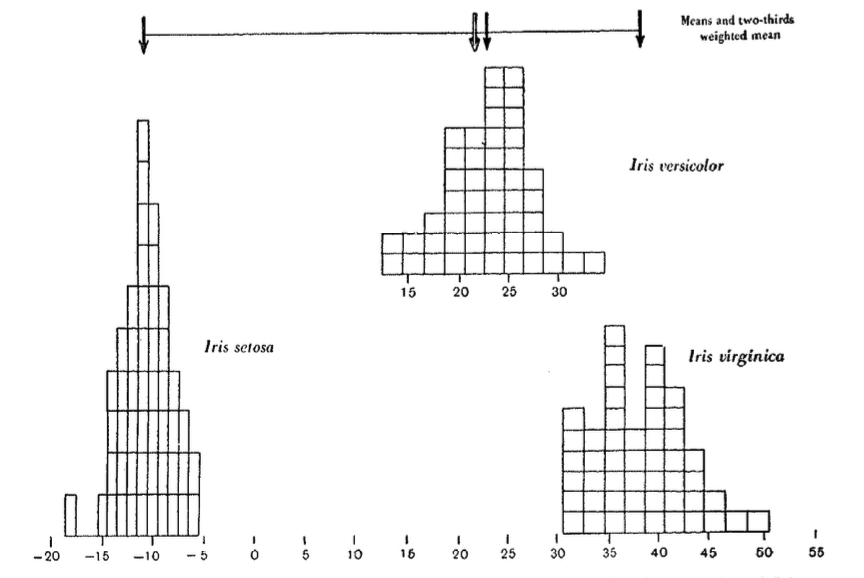
\includegraphics[width=1\linewidth]{img.png}
\caption{Frequency histograms of the discriminating linear function, for three species of \(Iris\).}
\label{fig:1}
\end{figure}

The diagram, Figure~\ref{fig:1}, shows the actual distributions of the compound measurement adopted in the individuals of the three species measured. It will be noticed, as was anticipated above, that there is some overlap of the distributions of \textit{I. virginica} and \textit{I. versicolor}, so that a certain diagnosis of these two species could not be based solely on these four measurements of a single flower taken on a plant growing wild. It is not, however, impossible that in culture the measurements alone should afford a more complete discrimination.

\section*{References}
\begin{itemize}
\item Randolph, L. F. (1934). ``Chromosome numbers in native American and introduced species and cultivated varieties of Iris.'' \textit{Bull. Amer. Iris Soc.} \textbf{52}, 61-66.
\item Anderson, Edgar (1935). ``The irises of the Gaspe Peninsula.'' \textit{Bull. Amer. Iris Soc.} \textbf{59}, 2-5.
\item Anderson, Edgar (1936). ``The species problem in \textit{Iris}.'' \textit{Ann. Mo. bot. Gdn.} (in the Press).
\end{itemize}

\end{document}